\documentclass[11pt,a4paper]{article}
\usepackage[margin=2.3cm]{geometry}
\usepackage[T1]{fontenc}
\usepackage{textcomp}
\input{glyphtounicode}
\pdfgentounicode=1
\usepackage{lmodern}
\usepackage{xcolor}
\usepackage{listings}
\usepackage{tcolorbox}
\usepackage{booktabs}
\usepackage{array}
\usepackage{tikz}
\usepackage{hyperref}
\hypersetup{colorlinks=true, linkcolor=blue!50!black, citecolor=green!40!black}

\definecolor{codebg}{RGB}{248,248,245}
\lstset{
  language=C, basicstyle=\ttfamily\footnotesize, backgroundcolor=\color{codebg},
  keywordstyle=\color{blue!60!black}\bfseries, commentstyle=\color{green!45!black}\itshape,
  stringstyle=\color{red!60!black}, numbers=none, upquote=true,
  frame=single, rulecolor=\color{gray!40}, breaklines=true, columns=fullflexible,
  keepspaces=true, showstringspaces=false, morekeywords={_Alignas}
}
\lstdefinestyle{sh}{language=bash, backgroundcolor=\color{black!5}}

\newtcolorbox{keyidea}{colback=blue!4, colframe=blue!45!black, title=Key ideas, fonttitle=\bfseries\small}
\newtcolorbox{experiment}{colback=orange!5, colframe=orange!70!black, title=Experiment, fonttitle=\bfseries\small}

\title{\textbf{OpenMP --- Lesson 8}\\[4pt]\large False sharing}
\author{Gustavo Lozano}
\date{November 2026}

\begin{document}
\maketitle

\noindent\textit{\small Source: Chapman, Jost \& van der Pas~\cite{chapman}, Ch.~5
``How to Get Good Performance'' (false sharing).}

\section{The idea}
Lessons 2--7 were about \emph{correctness}. This lesson is about \emph{speed}, and it
shows a problem that the source code does not reveal.

A CPU core does not read single bytes from memory. It copies a whole \textbf{cache line},
usually 64 bytes, into its private cache. When a core \emph{writes} to a line, the
hardware must invalidate every other core's copy of that line, so that no core keeps a
stale value. This is called \emph{cache coherence}.

Now let each thread increment its own counter, \texttt{packed[id]}. There is \textbf{no
data race}: no two threads touch the same variable. But 8 \texttt{long}s fit in one 64-byte
line, so all the counters live in the \emph{same} line. Every write by thread 0 invalidates
the line in thread 1's cache and vice versa. The line bounces between the cores on every
increment. This is \textbf{false sharing}: the threads share a cache line, not data.

\begin{center}
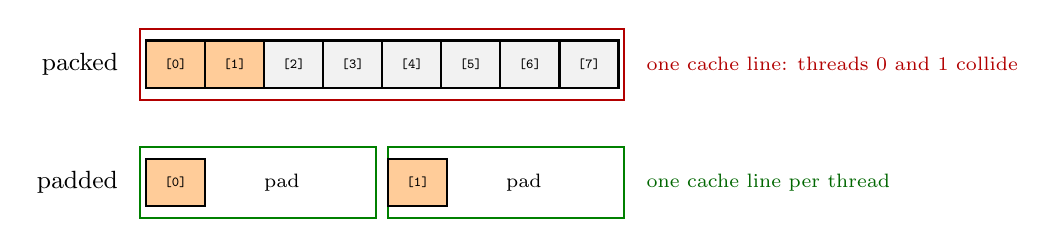
\begin{tikzpicture}[thick, x=0.75cm]
  \node[font=\small, anchor=east] at (-0.3,0.3) {packed};
  \draw[red!70!black] (-0.1,-0.15) rectangle (8.1,0.75);
  \foreach \i in {0,...,7} {
    \pgfmathsetmacro{\c}{\i<2 ? "orange!40" : "gray!10"}
    \node[draw, fill=\c, minimum width=0.75cm, minimum height=0.6cm, font=\tiny\ttfamily] at (\i+0.5,0.3) {[\i]};
  }
  \node[font=\scriptsize, red!70!black, anchor=west] at (8.3,0.3) {one cache line: threads 0 and 1 collide};
  \node[font=\small, anchor=east] at (-0.3,-1.2) {padded};
  \draw[green!50!black] (-0.1,-1.65) rectangle (3.9,-0.75);
  \draw[green!50!black] (4.1,-1.65) rectangle (8.1,-0.75);
  \node[draw, fill=orange!40, minimum width=0.75cm, minimum height=0.6cm, font=\tiny\ttfamily] at (0.5,-1.2) {[0]};
  \node[draw, fill=orange!40, minimum width=0.75cm, minimum height=0.6cm, font=\tiny\ttfamily] at (4.6,-1.2) {[1]};
  \node[font=\scriptsize] at (2.3,-1.2) {pad};
  \node[font=\scriptsize] at (6.4,-1.2) {pad};
  \node[font=\scriptsize, green!40!black, anchor=west] at (8.3,-1.2) {one cache line per thread};
\end{tikzpicture}
\end{center}

\section{Two fixes}
\begin{center}
\small
\begin{tabular}{@{}>{\raggedright\arraybackslash}p{3.2cm}>{\raggedright\arraybackslash}p{12.0cm}@{}}
\toprule
Fix & How \\ \midrule
\textbf{Padding} & make each thread's element occupy a whole cache line, e.g.\ with
  C11 \texttt{\_Alignas(64)}, so different threads never write the same line \\
\textbf{Local variable} & accumulate in a variable private to the thread (it lives in a
  register or on that thread's stack) and write the shared array \emph{once} at the end.
  This is what \texttt{reduction} does for you (Lesson~3) \\
\bottomrule
\end{tabular}
\end{center}

\section{The code}
The same work three times: each thread does $10^8$ increments of its own counter.
\lstinputlisting[title=\texttt{false\_sharing.c}]{false_sharing.c}

\begin{lstlisting}[style=sh]
gcc -Wall -fopenmp -o false_sharing false_sharing.c
OMP_NUM_THREADS=2 ./false_sharing
\end{lstlisting}
Output on a 2-core machine (your times will differ):
\begin{lstlisting}[style=sh]
threads = 2, sizeof(padded_t) = 64 bytes

packed : 0.423 s
padded : 0.200 s
local  : 0.042 s
\end{lstlisting}

\begin{keyidea}
\begin{itemize}
  \item All three versions are \emph{correct}: no thread ever touches another thread's
        counter. They differ only in memory layout.
  \item Each thread does the same work in every version, so with enough cores the time
        should not depend on the number of threads. \texttt{packed} breaks this rule: it
        gets slower as threads are added.
  \item False sharing is invisible in the source code. You find it by measuring, and by
        asking: do threads \emph{write} to addresses closer than 64 bytes apart?
  \item Reading is not the problem. Only writes force the other copies to be invalidated.
\end{itemize}
\end{keyidea}

\section{The experiment}
\begin{experiment}
\textbf{Question:} how does false sharing scale with the number of threads?
\begin{enumerate}
  \item Check your cache line size and number of cores:
\begin{lstlisting}[style=sh]
getconf LEVEL1_DCACHE_LINESIZE
nproc
\end{lstlisting}
  \item Run with every thread count from 1 up to \texttt{nproc}:
\begin{lstlisting}[style=sh]
for t in $(seq 1 $(nproc)); do echo "== $t"; OMP_NUM_THREADS=$t ./false_sharing | tail -3; done
\end{lstlisting}
  \item Write a table: rows = thread count, columns = \texttt{packed}, \texttt{padded},
        \texttt{local}.
\end{enumerate}
\textbf{What to observe and answer.}
\begin{enumerate}
  \item With 1 thread, \texttt{packed} and \texttt{padded} take the same time. Why?
  \item How does \texttt{packed} change as threads are added? And \texttt{padded}?
  \item Why is \texttt{local} the fastest, even with 1 thread?
\end{enumerate}
\end{experiment}

\paragraph{Answers (read after trying).}
(1)~With one thread no other core holds a copy of the line, so nothing is invalidated.
Both versions do the same instructions.
(2)~\texttt{packed} slows down: every extra thread writing into the same line adds more
invalidations and transfers between cores (on the 2-core test machine it went from 0.20\,s
to 0.42\,s). \texttt{padded} stays roughly constant, which is the ideal behaviour when each
thread has a fixed amount of independent work.
(3)~Every iteration of \texttt{packed} and \texttt{padded} must compute an address in a
global array and update it. \texttt{local} only updates a private variable that no other
core ever touches, so it stays in this core's cache, and the shared array is written once.
It avoids false sharing \emph{and} the indexing work. Rule: accumulate privately, write shared data rarely.

\paragraph{Next lesson.} Locks and \texttt{ordered}: protecting shared data with the lock
routines of the OpenMP library, and forcing part of a parallel loop to run in sequential
order (Chapman et al., Ch.~4).

\begin{thebibliography}{9}
\bibitem{chapman} B.~Chapman, G.~Jost, and R.~van der Pas. \emph{Using OpenMP: Portable
  Shared Memory Parallel Programming}. MIT Press, Cambridge, MA, 2007.
\end{thebibliography}
\end{document}
